\documentclass[1p]{elsarticle_modified}
%\bibliographystyle{elsarticle-num}

%\usepackage[colorlinks]{hyperref}
%\usepackage{abbrmath_seonhwa} %\Abb, \Ascr, \Acal ,\Abf, \Afrak
\usepackage{amsfonts}
\usepackage{amssymb}
\usepackage{amsmath}
\usepackage{amsthm}
\usepackage{scalefnt}
\usepackage{amsbsy}
\usepackage{kotex}
\usepackage{caption}
\usepackage{subfig}
\usepackage{color}
\usepackage{graphicx}
\usepackage{xcolor} %% white, black, red, green, blue, cyan, magenta, yellow
\usepackage{float}
\usepackage{setspace}
\usepackage{hyperref}

\usepackage{tikz}
\usetikzlibrary{arrows}

\usepackage{multirow}
\usepackage{array} % fixed length table
\usepackage{hhline}

%%%%%%%%%%%%%%%%%%%%%
\makeatletter
\renewcommand*\env@matrix[1][\arraystretch]{%
	\edef\arraystretch{#1}%
	\hskip -\arraycolsep
	\let\@ifnextchar\new@ifnextchar
	\array{*\c@MaxMatrixCols c}}
\makeatother %https://tex.stackexchange.com/questions/14071/how-can-i-increase-the-line-spacing-in-a-matrix
%%%%%%%%%%%%%%%

\usepackage[normalem]{ulem}

\newcommand{\msout}[1]{\ifmmode\text{\sout{\ensuremath{#1}}}\else\sout{#1}\fi}
%SOURCE: \msout is \stkout macro in https://tex.stackexchange.com/questions/20609/strikeout-in-math-mode

\newcommand{\cancel}[1]{
	\ifmmode
	{\color{red}\msout{#1}}
	\else
	{\color{red}\sout{#1}}
	\fi
}

\newcommand{\add}[1]{
	{\color{blue}\uwave{#1}}
}

\newcommand{\replace}[2]{
	\ifmmode
	{\color{red}\msout{#1}}{\color{blue}\uwave{#2}}
	\else
	{\color{red}\sout{#1}}{\color{blue}\uwave{#2}}
	\fi
}

\newcommand{\Sol}{\mathcal{S}} %segment
\newcommand{\D}{D} %diagram
\newcommand{\A}{\mathcal{A}} %arc


%%%%%%%%%%%%%%%%%%%%%%%%%%%%%5 test

\def\sl{\operatorname{\textup{SL}}(2,\Cbb)}
\def\psl{\operatorname{\textup{PSL}}(2,\Cbb)}
\def\quan{\mkern 1mu \triangleright \mkern 1mu}

\theoremstyle{definition}
\newtheorem{thm}{Theorem}[section]
\newtheorem{prop}[thm]{Proposition}
\newtheorem{lem}[thm]{Lemma}
\newtheorem{ques}[thm]{Question}
\newtheorem{cor}[thm]{Corollary}
\newtheorem{defn}[thm]{Definition}
\newtheorem{exam}[thm]{Example}
\newtheorem{rmk}[thm]{Remark}
\newtheorem{alg}[thm]{Algorithm}

\newcommand{\I}{\sqrt{-1}}
\begin{document}

%\begin{frontmatter}
%
%\title{Boundary parabolic representations of knots up to 8 crossings}
%
%%% Group authors per affiliation:
%\author{Yunhi Cho} 
%\address{Department of Mathematics, University of Seoul, Seoul, Korea}
%\ead{yhcho@uos.ac.kr}
%
%
%\author{Seonhwa Kim} %\fnref{s_kim}}
%\address{Center for Geometry and Physics, Institute for Basic Science, Pohang, 37673, Korea}
%\ead{ryeona17@ibs.re.kr}
%
%\author{Hyuk Kim}
%\address{Department of Mathematical Sciences, Seoul National University, Seoul 08826, Korea}
%\ead{hyukkim@snu.ac.kr}
%
%\author{Seokbeom Yoon}
%\address{Department of Mathematical Sciences, Seoul National University, Seoul, 08826,  Korea}
%\ead{sbyoon15@snu.ac.kr}
%
%\begin{abstract}
%We find all boundary parabolic representation of knots up to 8 crossings.
%
%\end{abstract}
%\begin{keyword}
%    \MSC[2010] 57M25 
%\end{keyword}
%
%\end{frontmatter}

%\linenumbers
%\tableofcontents
%
\newcommand\colored[1]{\textcolor{white}{\rule[-0.35ex]{0.8em}{1.4ex}}\kern-0.8em\color{red} #1}%
%\newcommand\colored[1]{\textcolor{white}{ #1}\kern-2.17ex	\textcolor{white}{ #1}\kern-1.81ex	\textcolor{white}{ #1}\kern-2.15ex\color{red}#1	}

{\Large $\underline{12a_{0939}~(K12a_{0939})}$}

\setlength{\tabcolsep}{10pt}
\renewcommand{\arraystretch}{1.6}
\vspace{1cm}\begin{tabular}{m{100pt}>{\centering\arraybackslash}m{274pt}}
\multirow{5}{120pt}{
	\centering
	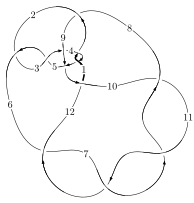
\includegraphics[width=112pt]{../../../GIT/diagram.site/Diagrams/png/1740_12a_0939.png}\\
\ \ \ A knot diagram\footnotemark}&
\allowdisplaybreaks
\textbf{Linearized knot diagam} \\
\cline{2-2}
 &
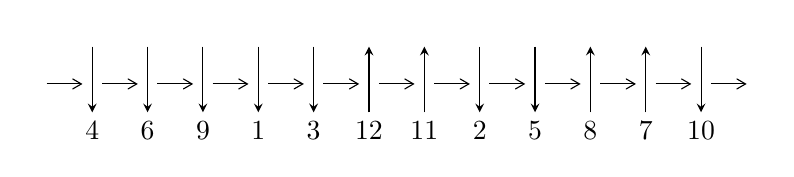
\begin{tikzpicture}[x=20pt, y=17pt]
	% nodes
	\node (C0) at (0, 0) {};
	\node (C1) at (1, 0) {};
	\node (C1U) at (1, +1) {};
	\node (C1D) at (1, -1) {4};

	\node (C2) at (2, 0) {};
	\node (C2U) at (2, +1) {};
	\node (C2D) at (2, -1) {6};

	\node (C3) at (3, 0) {};
	\node (C3U) at (3, +1) {};
	\node (C3D) at (3, -1) {9};

	\node (C4) at (4, 0) {};
	\node (C4U) at (4, +1) {};
	\node (C4D) at (4, -1) {1};

	\node (C5) at (5, 0) {};
	\node (C5U) at (5, +1) {};
	\node (C5D) at (5, -1) {3};

	\node (C6) at (6, 0) {};
	\node (C6U) at (6, +1) {};
	\node (C6D) at (6, -1) {12};

	\node (C7) at (7, 0) {};
	\node (C7U) at (7, +1) {};
	\node (C7D) at (7, -1) {11};

	\node (C8) at (8, 0) {};
	\node (C8U) at (8, +1) {};
	\node (C8D) at (8, -1) {2};

	\node (C9) at (9, 0) {};
	\node (C9U) at (9, +1) {};
	\node (C9D) at (9, -1) {5};

	\node (C10) at (10, 0) {};
	\node (C10U) at (10, +1) {};
	\node (C10D) at (10, -1) {8};

	\node (C11) at (11, 0) {};
	\node (C11U) at (11, +1) {};
	\node (C11D) at (11, -1) {7};

	\node (C12) at (12, 0) {};
	\node (C12U) at (12, +1) {};
	\node (C12D) at (12, -1) {10};
	\node (C13) at (13, 0) {};

	% arrows
	\draw[->,>={angle 60}]
	(C0) edge (C1) (C1) edge (C2) (C2) edge (C3) (C3) edge (C4) (C4) edge (C5) (C5) edge (C6) (C6) edge (C7) (C7) edge (C8) (C8) edge (C9) (C9) edge (C10) (C10) edge (C11) (C11) edge (C12) (C12) edge (C13) ;	\draw[->,>=stealth]
	(C1U) edge (C1D) (C2U) edge (C2D) (C3U) edge (C3D) (C4U) edge (C4D) (C5U) edge (C5D) (C6D) edge (C6U) (C7D) edge (C7U) (C8U) edge (C8D) (C9U) edge (C9D) (C10D) edge (C10U) (C11D) edge (C11U) (C12U) edge (C12D) ;
	\end{tikzpicture} \\
\hhline{~~} \\& 
\textbf{Solving Sequence} \\ \cline{2-2} 
 &
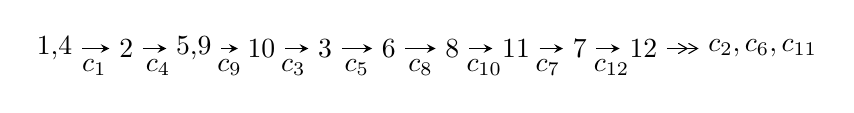
\begin{tikzpicture}[x=23pt, y=7pt]
	% node
	\node (A0) at (-1/8, 0) {1,4};
	\node (A1) at (1, 0) {2};
	\node (A2) at (33/16, 0) {5,9};
	\node (A3) at (25/8, 0) {10};
	\node (A4) at (33/8, 0) {3};
	\node (A5) at (41/8, 0) {6};
	\node (A6) at (49/8, 0) {8};
	\node (A7) at (57/8, 0) {11};
	\node (A8) at (65/8, 0) {7};
	\node (A9) at (73/8, 0) {12};
	\node (C1) at (1/2, -1) {$c_{1}$};
	\node (C2) at (3/2, -1) {$c_{4}$};
	\node (C3) at (21/8, -1) {$c_{9}$};
	\node (C4) at (29/8, -1) {$c_{3}$};
	\node (C5) at (37/8, -1) {$c_{5}$};
	\node (C6) at (45/8, -1) {$c_{8}$};
	\node (C7) at (53/8, -1) {$c_{10}$};
	\node (C8) at (61/8, -1) {$c_{7}$};
	\node (C9) at (69/8, -1) {$c_{12}$};
	\node (A10) at (11, 0) {$c_{2},c_{6},c_{11}$};

	% edge
	\draw[->,>=stealth]	
	(A0) edge (A1) (A1) edge (A2) (A2) edge (A3) (A3) edge (A4) (A4) edge (A5) (A5) edge (A6) (A6) edge (A7) (A7) edge (A8) (A8) edge (A9) ;
	\draw[->>,>={angle 60}]	
	(A9) edge (A10);
\end{tikzpicture} \\ 

\end{tabular} \\

\footnotetext{
The image of knot diagram is generated by the software ``\textbf{Draw programme}" developed by Andrew Bartholomew(\url{http://www.layer8.co.uk/maths/draw/index.htm\#Running-draw}), where we modified some parts for our purpose(\url{https://github.com/CATsTAILs/LinksPainter}).
}\phantom \\ \newline 
\centering \textbf{Ideals for irreducible components\footnotemark of $X_{\text{par}}$} 
 
\begin{align*}
I^u_{1}&=\langle 
8191 u^{30}-26107 u^{29}+\cdots+32768 b-33535,\;263 u^{30}-1185 u^{29}+\cdots+512 a-233,\\
\phantom{I^u_{1}}&\phantom{= \langle  }u^{31}-4 u^{30}+\cdots-6 u-1\rangle \\
I^u_{2}&=\langle 
-2.55785\times10^{49} u^{51}-2.68690\times10^{50} u^{50}+\cdots+5.56688\times10^{49} b-6.70004\times10^{48},\\
\phantom{I^u_{2}}&\phantom{= \langle  }-8.26170\times10^{49} u^{51}-6.92304\times10^{50} u^{50}+\cdots+5.56688\times10^{49} a-1.67397\times10^{49},\;u^{52}+9 u^{51}+\cdots+2 u+1\rangle \\
I^u_{3}&=\langle 
16 b^4-8 b^3+4 b^2+1,\;a,\;u-1\rangle \\
\\
\end{align*}
\raggedright * 3 irreducible components of $\dim_{\mathbb{C}}=0$, with total 87 representations.\\
\footnotetext{All coefficients of polynomials are rational numbers. But the coefficients are sometimes approximated in decimal forms when there is not enough margin.}
\newpage
\renewcommand{\arraystretch}{1}
\centering \section*{I. $I^u_{1}= \langle 8191 u^{30}-26107 u^{29}+\cdots+32768 b-33535,\;263 u^{30}-1185 u^{29}+\cdots+512 a-233,\;u^{31}-4 u^{30}+\cdots-6 u-1 \rangle$}
\flushleft \textbf{(i) Arc colorings}\\
\begin{tabular}{m{7pt} m{180pt} m{7pt} m{180pt} }
\flushright $a_{1}=$&$\begin{pmatrix}1\\0\end{pmatrix}$ \\
\flushright $a_{4}=$&$\begin{pmatrix}0\\u\end{pmatrix}$ \\
\flushright $a_{2}=$&$\begin{pmatrix}1\\u^2\end{pmatrix}$ \\
\flushright $a_{5}=$&$\begin{pmatrix}- u\\u\end{pmatrix}$ \\
\flushright $a_{9}=$&$\begin{pmatrix}-0.513672 u^{30}+2.31445 u^{29}+\cdots+9.14648 u+0.455078\\-0.249969 u^{30}+0.796722 u^{29}+\cdots+4.14828 u+1.02341\end{pmatrix}$ \\
\flushright $a_{10}=$&$\begin{pmatrix}-0.531281 u^{30}+2.21890 u^{29}+\cdots+9.57047 u+0.398468\\-0.232361 u^{30}+0.892273 u^{29}+\cdots+3.72430 u+1.08002\end{pmatrix}$ \\
\flushright $a_{3}=$&$\begin{pmatrix}-\frac{1}{4} u^{30}+\frac{3}{4} u^{29}+\cdots+\frac{7}{4} u+\frac{5}{4}\\\frac{1}{4} u^{30}-\frac{3}{4} u^{29}+\cdots-\frac{7}{4} u-\frac{1}{4}\end{pmatrix}$ \\
\flushright $a_{6}=$&$\begin{pmatrix}\frac{1}{4} u^{30}-\frac{5}{4} u^{29}+\cdots-\frac{3}{4} u+\frac{1}{4}\\-\frac{1}{4} u^{30}+\frac{5}{4} u^{29}+\cdots-\frac{1}{4} u-\frac{1}{4}\end{pmatrix}$ \\
\flushright $a_{8}=$&$\begin{pmatrix}-0.570282 u^{30}+2.52328 u^{29}+\cdots+12.2498 u+1.21872\\-0.415955 u^{30}+1.69305 u^{29}+\cdots+3.98602 u+1.00580\end{pmatrix}$ \\
\flushright $a_{11}=$&$\begin{pmatrix}-0.207794 u^{30}+1.06973 u^{29}+\cdots+1.39249 u-2.33078\\0.0252075 u^{30}-0.209045 u^{29}+\cdots+3.75287 u+0.573425\end{pmatrix}$ \\
\flushright $a_{7}=$&$\begin{pmatrix}0.253632 u^{30}-1.26767 u^{29}+\cdots+3.22989 u+0.245880\\-0.258606 u^{30}+1.29205 u^{29}+\cdots-0.203064 u-0.240417\end{pmatrix}$ \\
\flushright $a_{12}=$&$\begin{pmatrix}0.249969 u^{30}-1.24985 u^{29}+\cdots-1.74985 u+2.25003\\-0.249939 u^{30}+1.24969 u^{29}+\cdots-2.25031 u-0.250061\end{pmatrix}$\\&\end{tabular}
\flushleft \textbf{(ii) Obstruction class $= -1$}\\~\\
\flushleft \textbf{(iii) Cusp Shapes $= -\frac{77823}{65536} u^{30}+\frac{372731}{65536} u^{29}+\cdots+\frac{1036283}{65536} u+\frac{151551}{65536}$}\\~\\
\newpage\renewcommand{\arraystretch}{1}
\flushleft \textbf{(iv) u-Polynomials at the component}\newline \\
\begin{tabular}{m{50pt}|m{274pt}}
Crossings & \hspace{64pt}u-Polynomials at each crossing \\
\hline $$\begin{aligned}c_{1},c_{2},c_{4}\\c_{5}\end{aligned}$$&$\begin{aligned}
&u^{31}+4 u^{30}+\cdots-6 u+1
\end{aligned}$\\
\hline $$\begin{aligned}c_{3}\end{aligned}$$&$\begin{aligned}
&u^{31}+3 u^{30}+\cdots+1408 u+512
\end{aligned}$\\
\hline $$\begin{aligned}c_{6},c_{7},c_{10}\\c_{11}\end{aligned}$$&$\begin{aligned}
&u^{31}+17 u^{29}+\cdots+21 u+4
\end{aligned}$\\
\hline $$\begin{aligned}c_{8},c_{9}\end{aligned}$$&$\begin{aligned}
&16(16 u^{31}-8 u^{30}+\cdots+2 u+1)
\end{aligned}$\\
\hline $$\begin{aligned}c_{12}\end{aligned}$$&$\begin{aligned}
&u^{31}-6 u^{30}+\cdots+27315 u-4448
\end{aligned}$\\
\hline
\end{tabular}\\~\\
\newpage\renewcommand{\arraystretch}{1}
\flushleft \textbf{(v) Riley Polynomials at the component}\newline \\
\begin{tabular}{m{50pt}|m{274pt}}
Crossings & \hspace{64pt}Riley Polynomials at each crossing \\
\hline $$\begin{aligned}c_{1},c_{2},c_{4}\\c_{5}\end{aligned}$$&$\begin{aligned}
&y^{31}+16 y^{30}+\cdots+12 y-1
\end{aligned}$\\
\hline $$\begin{aligned}c_{3}\end{aligned}$$&$\begin{aligned}
&y^{31}+9 y^{30}+\cdots-4407296 y-262144
\end{aligned}$\\
\hline $$\begin{aligned}c_{6},c_{7},c_{10}\\c_{11}\end{aligned}$$&$\begin{aligned}
&y^{31}+34 y^{30}+\cdots+113 y-16
\end{aligned}$\\
\hline $$\begin{aligned}c_{8},c_{9}\end{aligned}$$&$\begin{aligned}
&256(256 y^{31}+3136 y^{30}+\cdots-8 y-1)
\end{aligned}$\\
\hline $$\begin{aligned}c_{12}\end{aligned}$$&$\begin{aligned}
&y^{31}+14 y^{30}+\cdots+1208087401 y-19784704
\end{aligned}$\\
\hline
\end{tabular}\\~\\
\newpage\flushleft \textbf{(vi) Complex Volumes and Cusp Shapes}
$$\begin{array}{c|c|c}  
\text{Solutions to }I^u_{1}& \I (\text{vol} + \sqrt{-1}CS) & \text{Cusp shape}\\
 \hline 
\begin{aligned}
u &= \phantom{-}0.800565 + 0.436099 I \\
a &= \phantom{-}0.467719 - 0.621707 I \\
b &= \phantom{-}0.042876 + 0.178508 I\end{aligned}
 & -2.45428 - 1.56605 I & -13.61992 + 2.18672 I \\ \hline\begin{aligned}
u &= \phantom{-}0.800565 - 0.436099 I \\
a &= \phantom{-}0.467719 + 0.621707 I \\
b &= \phantom{-}0.042876 - 0.178508 I\end{aligned}
 & -2.45428 + 1.56605 I & -13.61992 - 2.18672 I \\ \hline\begin{aligned}
u &= \phantom{-}0.939744 + 0.617749 I \\
a &= -0.276998 + 0.717790 I \\
b &= -0.195037 - 0.177639 I\end{aligned}
 & -9.79482 - 2.45438 I & -10.97758 + 0.07663 I \\ \hline\begin{aligned}
u &= \phantom{-}0.939744 - 0.617749 I \\
a &= -0.276998 - 0.717790 I \\
b &= -0.195037 + 0.177639 I\end{aligned}
 & -9.79482 + 2.45438 I & -10.97758 - 0.07663 I \\ \hline\begin{aligned}
u &= -0.402521 + 1.052770 I \\
a &= \phantom{-}1.48918 - 0.01324 I \\
b &= -2.36845 - 0.55108 I\end{aligned}
 & -6.57575 + 7.07387 I & -5.61246 - 7.92227 I \\ \hline\begin{aligned}
u &= -0.402521 - 1.052770 I \\
a &= \phantom{-}1.48918 + 0.01324 I \\
b &= -2.36845 + 0.55108 I\end{aligned}
 & -6.57575 - 7.07387 I & -5.61246 + 7.92227 I \\ \hline\begin{aligned}
u &= \phantom{-}0.107232 + 1.154900 I \\
a &= -0.99728 - 1.98978 I \\
b &= \phantom{-}1.52737 + 1.79295 I\end{aligned}
 & \phantom{-}5.77342 - 3.85223 I & \phantom{-}6.43651 + 8.75740 I \\ \hline\begin{aligned}
u &= \phantom{-}0.107232 - 1.154900 I \\
a &= -0.99728 + 1.98978 I \\
b &= \phantom{-}1.52737 - 1.79295 I\end{aligned}
 & \phantom{-}5.77342 + 3.85223 I & \phantom{-}6.43651 - 8.75740 I \\ \hline\begin{aligned}
u &= -0.031472 + 1.171320 I \\
a &= \phantom{-}1.78512 + 1.47159 I \\
b &= -2.36086 - 1.47488 I\end{aligned}
 & \phantom{-}7.04254 + 1.37301 I & \phantom{-}10.49996 - 3.37928 I \\ \hline\begin{aligned}
u &= -0.031472 - 1.171320 I \\
a &= \phantom{-}1.78512 - 1.47159 I \\
b &= -2.36086 + 1.47488 I\end{aligned}
 & \phantom{-}7.04254 - 1.37301 I & \phantom{-}10.49996 + 3.37928 I\\
 \hline 
 \end{array}$$\newpage$$\begin{array}{c|c|c}  
\text{Solutions to }I^u_{1}& \I (\text{vol} + \sqrt{-1}CS) & \text{Cusp shape}\\
 \hline 
\begin{aligned}
u &= \phantom{-}0.239386 + 1.151830 I \\
a &= \phantom{-}0.43439 + 1.74523 I \\
b &= -0.99450 - 1.41076 I\end{aligned}
 & -1.64522 - 7.50176 I & -1.21134 + 8.53156 I \\ \hline\begin{aligned}
u &= \phantom{-}0.239386 - 1.151830 I \\
a &= \phantom{-}0.43439 - 1.74523 I \\
b &= -0.99450 + 1.41076 I\end{aligned}
 & -1.64522 + 7.50176 I & -1.21134 - 8.53156 I \\ \hline\begin{aligned}
u &= -0.220760 + 1.161050 I \\
a &= -1.76111 - 0.50636 I \\
b &= \phantom{-}2.49381 + 0.76768 I\end{aligned}
 & \phantom{-}2.81930 + 5.65791 I & \phantom{-}0.15142 - 9.03827 I \\ \hline\begin{aligned}
u &= -0.220760 - 1.161050 I \\
a &= -1.76111 + 0.50636 I \\
b &= \phantom{-}2.49381 - 0.76768 I\end{aligned}
 & \phantom{-}2.81930 - 5.65791 I & \phantom{-}0.15142 + 9.03827 I \\ \hline\begin{aligned}
u &= \phantom{-}1.288550 + 0.093987 I \\
a &= \phantom{-}0.043092 - 0.447446 I \\
b &= \phantom{-}0.0329599 - 0.0695309 I\end{aligned}
 & -1.04564 + 1.63981 I & \phantom{-}6.17963 - 7.92782 I \\ \hline\begin{aligned}
u &= \phantom{-}1.288550 - 0.093987 I \\
a &= \phantom{-}0.043092 + 0.447446 I \\
b &= \phantom{-}0.0329599 + 0.0695309 I\end{aligned}
 & -1.04564 - 1.63981 I & \phantom{-}6.17963 + 7.92782 I \\ \hline\begin{aligned}
u &= -0.374044 + 1.323230 I \\
a &= -1.254180 - 0.415556 I \\
b &= \phantom{-}2.28135 + 0.63320 I\end{aligned}
 & \phantom{-}3.67791 + 5.94522 I & -1.46633 - 3.99996 I \\ \hline\begin{aligned}
u &= -0.374044 - 1.323230 I \\
a &= -1.254180 + 0.415556 I \\
b &= \phantom{-}2.28135 - 0.63320 I\end{aligned}
 & \phantom{-}3.67791 - 5.94522 I & -1.46633 + 3.99996 I \\ \hline\begin{aligned}
u &= \phantom{-}1.362480 + 0.213737 I \\
a &= -0.065860 + 0.497813 I \\
b &= -0.0818984 + 0.0915721 I\end{aligned}
 & -7.91870 + 3.73515 I & -1.51291 - 6.54236 I \\ \hline\begin{aligned}
u &= \phantom{-}1.362480 - 0.213737 I \\
a &= -0.065860 - 0.497813 I \\
b &= -0.0818984 - 0.0915721 I\end{aligned}
 & -7.91870 - 3.73515 I & -1.51291 + 6.54236 I\\
 \hline 
 \end{array}$$\newpage$$\begin{array}{c|c|c}  
\text{Solutions to }I^u_{1}& \I (\text{vol} + \sqrt{-1}CS) & \text{Cusp shape}\\
 \hline 
\begin{aligned}
u &= \phantom{-}0.587473\phantom{ +0.000000I} \\
a &= -0.910340\phantom{ +0.000000I} \\
b &= \phantom{-}0.138975\phantom{ +0.000000I}\end{aligned}
 & -0.937510\phantom{ +0.000000I} & -9.83160\phantom{ +0.000000I} \\ \hline\begin{aligned}
u &= -0.46571 + 1.36110 I \\
a &= \phantom{-}1.146720 + 0.344361 I \\
b &= -2.28464 - 0.57619 I\end{aligned}
 & \phantom{-}8.82124 + 9.22714 I & \phantom{-0.000000 } 0. - 4.14697 I \\ \hline\begin{aligned}
u &= -0.46571 - 1.36110 I \\
a &= \phantom{-}1.146720 - 0.344361 I \\
b &= -2.28464 + 0.57619 I\end{aligned}
 & \phantom{-}8.82124 - 9.22714 I & \phantom{-0.000000 -}0. + 4.14697 I \\ \hline\begin{aligned}
u &= -0.51997 + 1.36983 I \\
a &= -1.102860 - 0.305056 I \\
b &= \phantom{-}2.29782 + 0.55309 I\end{aligned}
 & \phantom{-}7.8389 + 13.6494 I & \phantom{-0.000000 } 0. - 9.33794 I \\ \hline\begin{aligned}
u &= -0.51997 - 1.36983 I \\
a &= -1.102860 + 0.305056 I \\
b &= \phantom{-}2.29782 - 0.55309 I\end{aligned}
 & \phantom{-}7.8389 - 13.6494 I & \phantom{-0.000000 -}0. + 9.33794 I \\ \hline\begin{aligned}
u &= -0.56513 + 1.37037 I \\
a &= \phantom{-}1.072670 + 0.273505 I \\
b &= -2.31235 - 0.53883 I\end{aligned}
 & \phantom{-}0.3710 + 16.6633 I & -4.00000 - 8.48351 I \\ \hline\begin{aligned}
u &= -0.56513 - 1.37037 I \\
a &= \phantom{-}1.072670 - 0.273505 I \\
b &= -2.31235 + 0.53883 I\end{aligned}
 & \phantom{-}0.3710 - 16.6633 I & -4.00000 + 8.48351 I \\ \hline\begin{aligned}
u &= -0.289932 + 0.249849 I \\
a &= \phantom{-}0.75811 - 1.38910 I \\
b &= -0.713923 - 0.779751 I\end{aligned}
 & -7.22830 - 2.70173 I & -3.88344 + 0.84995 I \\ \hline\begin{aligned}
u &= -0.289932 - 0.249849 I \\
a &= \phantom{-}0.75811 + 1.38910 I \\
b &= -0.713923 + 0.779751 I\end{aligned}
 & -7.22830 + 2.70173 I & -3.88344 - 0.84995 I \\ \hline\begin{aligned}
u &= -0.162159 + 0.123669 I \\
a &= -0.78355 + 2.04524 I \\
b &= \phantom{-}0.315969 + 0.529227 I\end{aligned}
 & -0.035297 - 1.217330 I & -0.51919 + 5.04787 I\\
 \hline 
 \end{array}$$\newpage$$\begin{array}{c|c|c}  
\text{Solutions to }I^u_{1}& \I (\text{vol} + \sqrt{-1}CS) & \text{Cusp shape}\\
 \hline 
\begin{aligned}
u &= -0.162159 - 0.123669 I \\
a &= -0.78355 - 2.04524 I \\
b &= \phantom{-}0.315969 - 0.529227 I\end{aligned}
 & -0.035297 + 1.217330 I & -0.51919 - 5.04787 I\\
 \hline 
 \end{array}$$\newpage\newpage\renewcommand{\arraystretch}{1}
\centering \section*{II. $I^u_{2}= \langle -2.56\times10^{49} u^{51}-2.69\times10^{50} u^{50}+\cdots+5.57\times10^{49} b-6.70\times10^{48},\;-8.26\times10^{49} u^{51}-6.92\times10^{50} u^{50}+\cdots+5.57\times10^{49} a-1.67\times10^{49},\;u^{52}+9 u^{51}+\cdots+2 u+1 \rangle$}
\flushleft \textbf{(i) Arc colorings}\\
\begin{tabular}{m{7pt} m{180pt} m{7pt} m{180pt} }
\flushright $a_{1}=$&$\begin{pmatrix}1\\0\end{pmatrix}$ \\
\flushright $a_{4}=$&$\begin{pmatrix}0\\u\end{pmatrix}$ \\
\flushright $a_{2}=$&$\begin{pmatrix}1\\u^2\end{pmatrix}$ \\
\flushright $a_{5}=$&$\begin{pmatrix}- u\\u\end{pmatrix}$ \\
\flushright $a_{9}=$&$\begin{pmatrix}1.48408 u^{51}+12.4361 u^{50}+\cdots+0.432390 u+0.300702\\0.459476 u^{51}+4.82658 u^{50}+\cdots+1.54387 u+0.120355\end{pmatrix}$ \\
\flushright $a_{10}=$&$\begin{pmatrix}2.14845 u^{51}+18.8762 u^{50}+\cdots+1.91732 u+0.0713913\\-0.204897 u^{51}-1.61347 u^{50}+\cdots+0.0589368 u+0.349666\end{pmatrix}$ \\
\flushright $a_{3}=$&$\begin{pmatrix}-0.454836 u^{51}-3.70365 u^{50}+\cdots+0.118831 u-2.10367\\-1\end{pmatrix}$ \\
\flushright $a_{6}=$&$\begin{pmatrix}- u^{51}-9 u^{50}+\cdots-2 u-2\\0.389875 u^{51}+3.14977 u^{50}+\cdots-1.19399 u+0.454836\end{pmatrix}$ \\
\flushright $a_{8}=$&$\begin{pmatrix}1.71919 u^{51}+15.1586 u^{50}+\cdots+1.61912 u-0.499551\\-0.581045 u^{51}-4.87305 u^{50}+\cdots+0.0957750 u-0.486136\end{pmatrix}$ \\
\flushright $a_{11}=$&$\begin{pmatrix}2.21012 u^{51}+19.1322 u^{50}+\cdots+1.52373 u+0.737565\\0.0271207 u^{51}+0.332337 u^{50}+\cdots-0.0316556 u+0.591378\end{pmatrix}$ \\
\flushright $a_{7}=$&$\begin{pmatrix}0.374845 u^{51}+3.05555 u^{50}+\cdots-0.280563 u-1.56949\\0.163327 u^{51}+1.34419 u^{50}+\cdots+0.258641 u+0.309612\end{pmatrix}$ \\
\flushright $a_{12}=$&$\begin{pmatrix}-1.73325 u^{51}-14.9638 u^{50}+\cdots-1.02224 u-0.206327\\0.0199941 u^{51}-0.206960 u^{50}+\cdots-0.299254 u-0.214321\end{pmatrix}$\\&\end{tabular}
\flushleft \textbf{(ii) Obstruction class $= -1$}\\~\\
\flushleft \textbf{(iii) Cusp Shapes $= -0.177316 u^{51}-0.0575527 u^{50}+\cdots-3.07266 u-2.10781$}\\~\\
\newpage\renewcommand{\arraystretch}{1}
\flushleft \textbf{(iv) u-Polynomials at the component}\newline \\
\begin{tabular}{m{50pt}|m{274pt}}
Crossings & \hspace{64pt}u-Polynomials at each crossing \\
\hline $$\begin{aligned}c_{1},c_{2},c_{4}\\c_{5}\end{aligned}$$&$\begin{aligned}
&u^{52}-9 u^{51}+\cdots-2 u+1
\end{aligned}$\\
\hline $$\begin{aligned}c_{3}\end{aligned}$$&$\begin{aligned}
&(u^{26}- u^{25}+\cdots- u+1)^{2}
\end{aligned}$\\
\hline $$\begin{aligned}c_{6},c_{7},c_{10}\\c_{11}\end{aligned}$$&$\begin{aligned}
&(u^{26}+u^{25}+\cdots- u+1)^{2}
\end{aligned}$\\
\hline $$\begin{aligned}c_{8},c_{9}\end{aligned}$$&$\begin{aligned}
&u^{52}- u^{51}+\cdots+307498 u+234119
\end{aligned}$\\
\hline $$\begin{aligned}c_{12}\end{aligned}$$&$\begin{aligned}
&(u^{26}-5 u^{25}+\cdots-5 u+3)^{2}
\end{aligned}$\\
\hline
\end{tabular}\\~\\
\newpage\renewcommand{\arraystretch}{1}
\flushleft \textbf{(v) Riley Polynomials at the component}\newline \\
\begin{tabular}{m{50pt}|m{274pt}}
Crossings & \hspace{64pt}Riley Polynomials at each crossing \\
\hline $$\begin{aligned}c_{1},c_{2},c_{4}\\c_{5}\end{aligned}$$&$\begin{aligned}
&y^{52}+35 y^{51}+\cdots-22 y^2+1
\end{aligned}$\\
\hline $$\begin{aligned}c_{3}\end{aligned}$$&$\begin{aligned}
&(y^{26}+9 y^{25}+\cdots+5 y+1)^{2}
\end{aligned}$\\
\hline $$\begin{aligned}c_{6},c_{7},c_{10}\\c_{11}\end{aligned}$$&$\begin{aligned}
&(y^{26}+29 y^{25}+\cdots+5 y+1)^{2}
\end{aligned}$\\
\hline $$\begin{aligned}c_{8},c_{9}\end{aligned}$$&$\begin{aligned}
&y^{52}+27 y^{51}+\cdots+786128549344 y+54811706161
\end{aligned}$\\
\hline $$\begin{aligned}c_{12}\end{aligned}$$&$\begin{aligned}
&(y^{26}+13 y^{25}+\cdots+161 y+9)^{2}
\end{aligned}$\\
\hline
\end{tabular}\\~\\
\newpage\flushleft \textbf{(vi) Complex Volumes and Cusp Shapes}
$$\begin{array}{c|c|c}  
\text{Solutions to }I^u_{2}& \I (\text{vol} + \sqrt{-1}CS) & \text{Cusp shape}\\
 \hline 
\begin{aligned}
u &= -0.918656 + 0.362726 I \\
a &= \phantom{-}0.880173 - 0.718377 I \\
b &= -0.246680 + 0.221124 I\end{aligned}
 & -1.37714 + 1.77746 I & \phantom{-0.000000 } 0 \\ \hline\begin{aligned}
u &= -0.918656 - 0.362726 I \\
a &= \phantom{-}0.880173 + 0.718377 I \\
b &= -0.246680 - 0.221124 I\end{aligned}
 & -1.37714 - 1.77746 I & \phantom{-0.000000 } 0 \\ \hline\begin{aligned}
u &= -1.019230 + 0.119379 I \\
a &= -0.732005 + 0.889313 I \\
b &= \phantom{-}0.0937238 - 0.0409991 I\end{aligned}
 & \phantom{-}4.21235 + 4.00629 I & \phantom{-0.000000 } 0 \\ \hline\begin{aligned}
u &= -1.019230 - 0.119379 I \\
a &= -0.732005 - 0.889313 I \\
b &= \phantom{-}0.0937238 + 0.0409991 I\end{aligned}
 & \phantom{-}4.21235 - 4.00629 I & \phantom{-0.000000 } 0 \\ \hline\begin{aligned}
u &= \phantom{-}0.529993 + 0.937993 I \\
a &= \phantom{-}1.051030 - 0.221738 I \\
b &= -1.48213 + 0.45619 I\end{aligned}
 & -8.60065 - 2.88146 I & \phantom{-0.000000 } 0 \\ \hline\begin{aligned}
u &= \phantom{-}0.529993 - 0.937993 I \\
a &= \phantom{-}1.051030 + 0.221738 I \\
b &= -1.48213 - 0.45619 I\end{aligned}
 & -8.60065 + 2.88146 I & \phantom{-0.000000 } 0 \\ \hline\begin{aligned}
u &= -0.098395 + 1.086290 I \\
a &= -0.518587 + 0.731973 I \\
b &= \phantom{-}1.42167 + 0.24596 I\end{aligned}
 & \phantom{-}2.31474 + 2.50037 I & \phantom{-0.000000 } 0 \\ \hline\begin{aligned}
u &= -0.098395 - 1.086290 I \\
a &= -0.518587 - 0.731973 I \\
b &= \phantom{-}1.42167 - 0.24596 I\end{aligned}
 & \phantom{-}2.31474 - 2.50037 I & \phantom{-0.000000 } 0 \\ \hline\begin{aligned}
u &= -0.200224 + 1.087680 I \\
a &= \phantom{-}0.444964 - 0.821616 I \\
b &= -1.263110 - 0.333811 I\end{aligned}
 & -4.97071 + 4.90123 I & \phantom{-0.000000 } 0 \\ \hline\begin{aligned}
u &= -0.200224 - 1.087680 I \\
a &= \phantom{-}0.444964 + 0.821616 I \\
b &= -1.263110 + 0.333811 I\end{aligned}
 & -4.97071 - 4.90123 I & \phantom{-0.000000 } 0\\
 \hline 
 \end{array}$$\newpage$$\begin{array}{c|c|c}  
\text{Solutions to }I^u_{2}& \I (\text{vol} + \sqrt{-1}CS) & \text{Cusp shape}\\
 \hline 
\begin{aligned}
u &= -1.107950 + 0.028133 I \\
a &= \phantom{-}0.633285 - 0.899169 I \\
b &= -0.0683414 - 0.0608682 I\end{aligned}
 & \phantom{-}3.43843 + 7.92757 I & \phantom{-0.000000 } 0 \\ \hline\begin{aligned}
u &= -1.107950 - 0.028133 I \\
a &= \phantom{-}0.633285 + 0.899169 I \\
b &= -0.0683414 + 0.0608682 I\end{aligned}
 & \phantom{-}3.43843 - 7.92757 I & \phantom{-0.000000 } 0 \\ \hline\begin{aligned}
u &= \phantom{-}0.335074 + 1.062310 I \\
a &= -0.914403 + 0.360247 I \\
b &= \phantom{-}1.52164 - 0.33683 I\end{aligned}
 & -0.43348 - 2.64715 I & \phantom{-0.000000 } 0 \\ \hline\begin{aligned}
u &= \phantom{-}0.335074 - 1.062310 I \\
a &= -0.914403 - 0.360247 I \\
b &= \phantom{-}1.52164 + 0.33683 I\end{aligned}
 & -0.43348 + 2.64715 I & \phantom{-0.000000 } 0 \\ \hline\begin{aligned}
u &= -0.023027 + 1.115250 I \\
a &= \phantom{-}0.385985 - 0.303188 I \\
b &= -2.70055 + 0.20079 I\end{aligned}
 & \phantom{-}3.35189 - 0.99254 I & \phantom{-0.000000 } 0 \\ \hline\begin{aligned}
u &= -0.023027 - 1.115250 I \\
a &= \phantom{-}0.385985 + 0.303188 I \\
b &= -2.70055 - 0.20079 I\end{aligned}
 & \phantom{-}3.35189 + 0.99254 I & \phantom{-0.000000 } 0 \\ \hline\begin{aligned}
u &= \phantom{-}0.015623 + 1.126090 I \\
a &= \phantom{-}0.584075 - 0.533445 I \\
b &= -1.70190 - 0.03427 I\end{aligned}
 & \phantom{-}3.17562 - 1.00551 I & \phantom{-0.000000 } 0 \\ \hline\begin{aligned}
u &= \phantom{-}0.015623 - 1.126090 I \\
a &= \phantom{-}0.584075 + 0.533445 I \\
b &= -1.70190 + 0.03427 I\end{aligned}
 & \phantom{-}3.17562 + 1.00551 I & \phantom{-0.000000 } 0 \\ \hline\begin{aligned}
u &= \phantom{-}0.242499 + 0.805416 I \\
a &= \phantom{-}0.116576 + 0.817043 I \\
b &= \phantom{-}1.13571 + 1.80548 I\end{aligned}
 & -3.13796 + 2.46970 I & -7.58807 - 2.77943 I \\ \hline\begin{aligned}
u &= \phantom{-}0.242499 - 0.805416 I \\
a &= \phantom{-}0.116576 - 0.817043 I \\
b &= \phantom{-}1.13571 - 1.80548 I\end{aligned}
 & -3.13796 - 2.46970 I & -7.58807 + 2.77943 I\\
 \hline 
 \end{array}$$\newpage$$\begin{array}{c|c|c}  
\text{Solutions to }I^u_{2}& \I (\text{vol} + \sqrt{-1}CS) & \text{Cusp shape}\\
 \hline 
\begin{aligned}
u &= -0.059936 + 0.827194 I \\
a &= -0.554765 - 0.357827 I \\
b &= \phantom{-}0.17463 - 2.28039 I\end{aligned}
 & \phantom{-}3.35189 + 0.99254 I & -2.96284 - 6.67512 I \\ \hline\begin{aligned}
u &= -0.059936 - 0.827194 I \\
a &= -0.554765 + 0.357827 I \\
b &= \phantom{-}0.17463 + 2.28039 I\end{aligned}
 & \phantom{-}3.35189 - 0.99254 I & -2.96284 + 6.67512 I \\ \hline\begin{aligned}
u &= -1.170810 + 0.041488 I \\
a &= -0.568970 - 0.897264 I \\
b &= \phantom{-}0.0500480 - 0.1320520 I\end{aligned}
 & -3.82921 - 10.57850 I & \phantom{-0.000000 } 0 \\ \hline\begin{aligned}
u &= -1.170810 - 0.041488 I \\
a &= -0.568970 + 0.897264 I \\
b &= \phantom{-}0.0500480 + 0.1320520 I\end{aligned}
 & -3.82921 + 10.57850 I & \phantom{-0.000000 } 0 \\ \hline\begin{aligned}
u &= \phantom{-}0.068858 + 1.173240 I \\
a &= -0.279445 + 0.520393 I \\
b &= \phantom{-}2.10779 + 0.88556 I\end{aligned}
 & -3.13796 - 2.46970 I & \phantom{-0.000000 } 0 \\ \hline\begin{aligned}
u &= \phantom{-}0.068858 - 1.173240 I \\
a &= -0.279445 - 0.520393 I \\
b &= \phantom{-}2.10779 - 0.88556 I\end{aligned}
 & -3.13796 + 2.46970 I & \phantom{-0.000000 } 0 \\ \hline\begin{aligned}
u &= -0.698738 + 0.390612 I \\
a &= -0.30488 - 1.41316 I \\
b &= -0.425347 - 0.027800 I\end{aligned}
 & -8.60065 - 2.88146 I & -9.60306 + 2.87824 I \\ \hline\begin{aligned}
u &= -0.698738 - 0.390612 I \\
a &= -0.30488 + 1.41316 I \\
b &= -0.425347 + 0.027800 I\end{aligned}
 & -8.60065 + 2.88146 I & -9.60306 - 2.87824 I \\ \hline\begin{aligned}
u &= -0.583877 + 0.110063 I \\
a &= \phantom{-}0.87448 + 1.62178 I \\
b &= \phantom{-}0.317378 - 0.232077 I\end{aligned}
 & -0.43348 - 2.64715 I & -8.54618 + 3.67555 I \\ \hline\begin{aligned}
u &= -0.583877 - 0.110063 I \\
a &= \phantom{-}0.87448 - 1.62178 I \\
b &= \phantom{-}0.317378 + 0.232077 I\end{aligned}
 & -0.43348 + 2.64715 I & -8.54618 - 3.67555 I\\
 \hline 
 \end{array}$$\newpage$$\begin{array}{c|c|c}  
\text{Solutions to }I^u_{2}& \I (\text{vol} + \sqrt{-1}CS) & \text{Cusp shape}\\
 \hline 
\begin{aligned}
u &= \phantom{-}0.26012 + 1.43593 I \\
a &= -0.727197 + 0.249900 I \\
b &= \phantom{-}1.66512 - 0.35502 I\end{aligned}
 & -1.37714 - 1.77746 I & \phantom{-0.000000 } 0 \\ \hline\begin{aligned}
u &= \phantom{-}0.26012 - 1.43593 I \\
a &= -0.727197 - 0.249900 I \\
b &= \phantom{-}1.66512 + 0.35502 I\end{aligned}
 & -1.37714 + 1.77746 I & \phantom{-0.000000 } 0 \\ \hline\begin{aligned}
u &= \phantom{-}0.44108 + 1.39128 I \\
a &= \phantom{-}0.781571 - 0.212164 I \\
b &= -1.64968 + 0.38783 I\end{aligned}
 & \phantom{-}4.21235 - 4.00629 I & \phantom{-0.000000 } 0 \\ \hline\begin{aligned}
u &= \phantom{-}0.44108 - 1.39128 I \\
a &= \phantom{-}0.781571 + 0.212164 I \\
b &= -1.64968 - 0.38783 I\end{aligned}
 & \phantom{-}4.21235 + 4.00629 I & \phantom{-0.000000 } 0 \\ \hline\begin{aligned}
u &= -0.70545 + 1.30058 I \\
a &= \phantom{-}0.671732 - 0.288948 I \\
b &= -1.172470 + 0.380087 I\end{aligned}
 & \phantom{-}1.26907 + 4.47678 I & \phantom{-0.000000 } 0 \\ \hline\begin{aligned}
u &= -0.70545 - 1.30058 I \\
a &= \phantom{-}0.671732 + 0.288948 I \\
b &= -1.172470 - 0.380087 I\end{aligned}
 & \phantom{-}1.26907 - 4.47678 I & \phantom{-0.000000 } 0 \\ \hline\begin{aligned}
u &= -0.60226 + 1.35652 I \\
a &= -0.660919 + 0.268780 I \\
b &= \phantom{-}1.268500 - 0.415860 I\end{aligned}
 & \phantom{-}7.87691 + 1.94179 I & \phantom{-0.000000 } 0 \\ \hline\begin{aligned}
u &= -0.60226 - 1.35652 I \\
a &= -0.660919 - 0.268780 I \\
b &= \phantom{-}1.268500 + 0.415860 I\end{aligned}
 & \phantom{-}7.87691 - 1.94179 I & \phantom{-0.000000 } 0 \\ \hline\begin{aligned}
u &= \phantom{-}0.53710 + 1.39983 I \\
a &= -0.793041 + 0.178882 I \\
b &= \phantom{-}1.65515 - 0.41186 I\end{aligned}
 & \phantom{-}3.43843 - 7.92757 I & \phantom{-0.000000 } 0 \\ \hline\begin{aligned}
u &= \phantom{-}0.53710 - 1.39983 I \\
a &= -0.793041 - 0.178882 I \\
b &= \phantom{-}1.65515 + 0.41186 I\end{aligned}
 & \phantom{-}3.43843 + 7.92757 I & \phantom{-0.000000 } 0\\
 \hline 
 \end{array}$$\newpage$$\begin{array}{c|c|c}  
\text{Solutions to }I^u_{2}& \I (\text{vol} + \sqrt{-1}CS) & \text{Cusp shape}\\
 \hline 
\begin{aligned}
u &= -0.51689 + 1.42731 I \\
a &= \phantom{-}0.648075 - 0.258123 I \\
b &= -1.36159 + 0.41343 I\end{aligned}
 & \phantom{-}7.87691 - 1.94179 I & \phantom{-0.000000 } 0 \\ \hline\begin{aligned}
u &= -0.51689 - 1.42731 I \\
a &= \phantom{-}0.648075 + 0.258123 I \\
b &= -1.36159 - 0.41343 I\end{aligned}
 & \phantom{-}7.87691 + 1.94179 I & \phantom{-0.000000 } 0 \\ \hline\begin{aligned}
u &= \phantom{-}0.61099 + 1.40315 I \\
a &= \phantom{-}0.798709 - 0.153496 I \\
b &= -1.66142 + 0.43078 I\end{aligned}
 & -3.82921 - 10.57850 I & \phantom{-0.000000 } 0 \\ \hline\begin{aligned}
u &= \phantom{-}0.61099 - 1.40315 I \\
a &= \phantom{-}0.798709 + 0.153496 I \\
b &= -1.66142 - 0.43078 I\end{aligned}
 & -3.82921 + 10.57850 I & \phantom{-0.000000 } 0 \\ \hline\begin{aligned}
u &= \phantom{-}0.427010 + 0.044189 I \\
a &= \phantom{-}1.70872 - 1.69549 I \\
b &= -1.048330 - 0.899889 I\end{aligned}
 & -4.97071 - 4.90123 I & -7.70149 + 2.20839 I \\ \hline\begin{aligned}
u &= \phantom{-}0.427010 - 0.044189 I \\
a &= \phantom{-}1.70872 + 1.69549 I \\
b &= -1.048330 + 0.899889 I\end{aligned}
 & -4.97071 + 4.90123 I & -7.70149 - 2.20839 I \\ \hline\begin{aligned}
u &= -0.44590 + 1.51192 I \\
a &= -0.638031 + 0.253035 I \\
b &= \phantom{-}1.43809 - 0.38336 I\end{aligned}
 & \phantom{-}1.26907 - 4.47678 I & \phantom{-0.000000 } 0 \\ \hline\begin{aligned}
u &= -0.44590 - 1.51192 I \\
a &= -0.638031 - 0.253035 I \\
b &= \phantom{-}1.43809 + 0.38336 I\end{aligned}
 & \phantom{-}1.26907 + 4.47678 I & \phantom{-0.000000 } 0 \\ \hline\begin{aligned}
u &= -0.065431 + 0.334054 I \\
a &= -2.21650 - 1.39141 I \\
b &= -0.444808 - 1.021440 I\end{aligned}
 & \phantom{-}3.17562 + 1.00551 I & -1.57769 - 3.62739 I \\ \hline\begin{aligned}
u &= -0.065431 - 0.334054 I \\
a &= -2.21650 + 1.39141 I \\
b &= -0.444808 + 1.021440 I\end{aligned}
 & \phantom{-}3.17562 - 1.00551 I & -1.57769 + 3.62739 I\\
 \hline 
 \end{array}$$\newpage$$\begin{array}{c|c|c}  
\text{Solutions to }I^u_{2}& \I (\text{vol} + \sqrt{-1}CS) & \text{Cusp shape}\\
 \hline 
\begin{aligned}
u &= \phantom{-}0.248411 + 0.140739 I \\
a &= -1.17063 + 3.22092 I \\
b &= \phantom{-}0.876909 + 0.937890 I\end{aligned}
 & \phantom{-}2.31474 - 2.50037 I & -4.62782 + 3.68649 I \\ \hline\begin{aligned}
u &= \phantom{-}0.248411 - 0.140739 I \\
a &= -1.17063 - 3.22092 I \\
b &= \phantom{-}0.876909 - 0.937890 I\end{aligned}
 & \phantom{-}2.31474 + 2.50037 I & -4.62782 - 3.68649 I\\
 \hline 
 \end{array}$$\newpage\newpage\renewcommand{\arraystretch}{1}
\centering \section*{III. $I^u_{3}= \langle 16 b^4-8 b^3+4 b^2+1,\;a,\;u-1 \rangle$}
\flushleft \textbf{(i) Arc colorings}\\
\begin{tabular}{m{7pt} m{180pt} m{7pt} m{180pt} }
\flushright $a_{1}=$&$\begin{pmatrix}1\\0\end{pmatrix}$ \\
\flushright $a_{4}=$&$\begin{pmatrix}0\\1\end{pmatrix}$ \\
\flushright $a_{2}=$&$\begin{pmatrix}1\\1\end{pmatrix}$ \\
\flushright $a_{5}=$&$\begin{pmatrix}-1\\1\end{pmatrix}$ \\
\flushright $a_{9}=$&$\begin{pmatrix}0\\b\end{pmatrix}$ \\
\flushright $a_{10}=$&$\begin{pmatrix}- b\\2 b\end{pmatrix}$ \\
\flushright $a_{3}=$&$\begin{pmatrix}0\\1\end{pmatrix}$ \\
\flushright $a_{6}=$&$\begin{pmatrix}-1\\0\end{pmatrix}$ \\
\flushright $a_{8}=$&$\begin{pmatrix}b\\2 b\end{pmatrix}$ \\
\flushright $a_{11}=$&$\begin{pmatrix}4 b^3- b\\8 b^3+2 b\end{pmatrix}$ \\
\flushright $a_{7}=$&$\begin{pmatrix}-4 b^3-2 b^2-\frac{1}{2}\\8 b^3-4 b^2-1\end{pmatrix}$ \\
\flushright $a_{12}=$&$\begin{pmatrix}2 b^2+1\\-4 b^2\end{pmatrix}$\\&\end{tabular}
\flushleft \textbf{(ii) Obstruction class $= 1$}\\~\\
\flushleft \textbf{(iii) Cusp Shapes $= b^2-10$}\\~\\
\newpage\renewcommand{\arraystretch}{1}
\flushleft \textbf{(iv) u-Polynomials at the component}\newline \\
\begin{tabular}{m{50pt}|m{274pt}}
Crossings & \hspace{64pt}u-Polynomials at each crossing \\
\hline $$\begin{aligned}c_{1},c_{2}\end{aligned}$$&$\begin{aligned}
&(u-1)^4
\end{aligned}$\\
\hline $$\begin{aligned}c_{3}\end{aligned}$$&$\begin{aligned}
&u^4
\end{aligned}$\\
\hline $$\begin{aligned}c_{4},c_{5}\end{aligned}$$&$\begin{aligned}
&(u+1)^4
\end{aligned}$\\
\hline $$\begin{aligned}c_{6},c_{7}\end{aligned}$$&$\begin{aligned}
&u^4+u^3+3 u^2+2 u+1
\end{aligned}$\\
\hline $$\begin{aligned}c_{8}\end{aligned}$$&$\begin{aligned}
&16(16 u^4+8 u^3+4 u^2+1)
\end{aligned}$\\
\hline $$\begin{aligned}c_{9}\end{aligned}$$&$\begin{aligned}
&16(16 u^4-8 u^3+4 u^2+1)
\end{aligned}$\\
\hline $$\begin{aligned}c_{10},c_{11}\end{aligned}$$&$\begin{aligned}
&u^4- u^3+3 u^2-2 u+1
\end{aligned}$\\
\hline $$\begin{aligned}c_{12}\end{aligned}$$&$\begin{aligned}
&u^4- u^3+u^2+1
\end{aligned}$\\
\hline
\end{tabular}\\~\\
\newpage\renewcommand{\arraystretch}{1}
\flushleft \textbf{(v) Riley Polynomials at the component}\newline \\
\begin{tabular}{m{50pt}|m{274pt}}
Crossings & \hspace{64pt}Riley Polynomials at each crossing \\
\hline $$\begin{aligned}c_{1},c_{2},c_{4}\\c_{5}\end{aligned}$$&$\begin{aligned}
&(y-1)^4
\end{aligned}$\\
\hline $$\begin{aligned}c_{3}\end{aligned}$$&$\begin{aligned}
&y^4
\end{aligned}$\\
\hline $$\begin{aligned}c_{6},c_{7},c_{10}\\c_{11}\end{aligned}$$&$\begin{aligned}
&y^4+5 y^3+7 y^2+2 y+1
\end{aligned}$\\
\hline $$\begin{aligned}c_{8},c_{9}\end{aligned}$$&$\begin{aligned}
&256(256 y^4+64 y^3+48 y^2+8 y+1)
\end{aligned}$\\
\hline $$\begin{aligned}c_{12}\end{aligned}$$&$\begin{aligned}
&y^4+y^3+3 y^2+2 y+1
\end{aligned}$\\
\hline
\end{tabular}\\~\\
\newpage\flushleft \textbf{(vi) Complex Volumes and Cusp Shapes}
$$\begin{array}{c|c|c}  
\text{Solutions to }I^u_{3}& \I (\text{vol} + \sqrt{-1}CS) & \text{Cusp shape}\\
 \hline 
\begin{aligned}
u &= \phantom{-}1.00000\phantom{ +0.000000I} \\
a &= \phantom{-0.000000 } 0 \\
b &= \phantom{-}0.425904 + 0.455646 I\end{aligned}
 & -8.43568 - 3.16396 I & -10.02622 + 0.38812 I \\ \hline\begin{aligned}
u &= \phantom{-}1.00000\phantom{ +0.000000I} \\
a &= \phantom{-0.000000 } 0 \\
b &= \phantom{-}0.425904 - 0.455646 I\end{aligned}
 & -8.43568 + 3.16396 I & -10.02622 - 0.38812 I \\ \hline\begin{aligned}
u &= \phantom{-}1.00000\phantom{ +0.000000I} \\
a &= \phantom{-0.000000 } 0 \\
b &= -0.175904 + 0.360171 I\end{aligned}
 & -1.43393 + 1.41510 I & -10.09878 - 0.12671 I \\ \hline\begin{aligned}
u &= \phantom{-}1.00000\phantom{ +0.000000I} \\
a &= \phantom{-0.000000 } 0 \\
b &= -0.175904 - 0.360171 I\end{aligned}
 & -1.43393 - 1.41510 I & -10.09878 + 0.12671 I\\
 \hline 
 \end{array}$$\newpage
\newpage\renewcommand{\arraystretch}{1}
\centering \section*{ IV. u-Polynomials}
\begin{tabular}{m{50pt}|m{274pt}}
Crossings & \hspace{64pt}u-Polynomials at each crossing \\
\hline $$\begin{aligned}c_{1},c_{2}\end{aligned}$$&$\begin{aligned}
&((u-1)^4)(u^{31}+4 u^{30}+\cdots-6 u+1)(u^{52}-9 u^{51}+\cdots-2 u+1)
\end{aligned}$\\
\hline $$\begin{aligned}c_{3}\end{aligned}$$&$\begin{aligned}
&u^4(u^{26}- u^{25}+\cdots- u+1)^{2}(u^{31}+3 u^{30}+\cdots+1408 u+512)
\end{aligned}$\\
\hline $$\begin{aligned}c_{4},c_{5}\end{aligned}$$&$\begin{aligned}
&((u+1)^4)(u^{31}+4 u^{30}+\cdots-6 u+1)(u^{52}-9 u^{51}+\cdots-2 u+1)
\end{aligned}$\\
\hline $$\begin{aligned}c_{6},c_{7}\end{aligned}$$&$\begin{aligned}
&(u^4+u^3+3 u^2+2 u+1)(u^{26}+u^{25}+\cdots- u+1)^{2}\\
&\cdot(u^{31}+17 u^{29}+\cdots+21 u+4)
\end{aligned}$\\
\hline $$\begin{aligned}c_{8}\end{aligned}$$&$\begin{aligned}
&256(16 u^4+8 u^3+4 u^2+1)(16 u^{31}-8 u^{30}+\cdots+2 u+1)\\
&\cdot(u^{52}- u^{51}+\cdots+307498 u+234119)
\end{aligned}$\\
\hline $$\begin{aligned}c_{9}\end{aligned}$$&$\begin{aligned}
&256(16 u^4-8 u^3+4 u^2+1)(16 u^{31}-8 u^{30}+\cdots+2 u+1)\\
&\cdot(u^{52}- u^{51}+\cdots+307498 u+234119)
\end{aligned}$\\
\hline $$\begin{aligned}c_{10},c_{11}\end{aligned}$$&$\begin{aligned}
&(u^4- u^3+3 u^2-2 u+1)(u^{26}+u^{25}+\cdots- u+1)^{2}\\
&\cdot(u^{31}+17 u^{29}+\cdots+21 u+4)
\end{aligned}$\\
\hline $$\begin{aligned}c_{12}\end{aligned}$$&$\begin{aligned}
&(u^4- u^3+u^2+1)(u^{26}-5 u^{25}+\cdots-5 u+3)^{2}\\
&\cdot(u^{31}-6 u^{30}+\cdots+27315 u-4448)
\end{aligned}$\\
\hline
\end{tabular}\newpage\renewcommand{\arraystretch}{1}
\centering \section*{ V. Riley Polynomials}
\begin{tabular}{m{50pt}|m{274pt}}
Crossings & \hspace{64pt}Riley Polynomials at each crossing \\
\hline $$\begin{aligned}c_{1},c_{2},c_{4}\\c_{5}\end{aligned}$$&$\begin{aligned}
&((y-1)^4)(y^{31}+16 y^{30}+\cdots+12 y-1)(y^{52}+35 y^{51}+\cdots-22 y^2+1)
\end{aligned}$\\
\hline $$\begin{aligned}c_{3}\end{aligned}$$&$\begin{aligned}
&y^4(y^{26}+9 y^{25}+\cdots+5 y+1)^{2}\\
&\cdot(y^{31}+9 y^{30}+\cdots-4407296 y-262144)
\end{aligned}$\\
\hline $$\begin{aligned}c_{6},c_{7},c_{10}\\c_{11}\end{aligned}$$&$\begin{aligned}
&(y^4+5 y^3+7 y^2+2 y+1)(y^{26}+29 y^{25}+\cdots+5 y+1)^{2}\\
&\cdot(y^{31}+34 y^{30}+\cdots+113 y-16)
\end{aligned}$\\
\hline $$\begin{aligned}c_{8},c_{9}\end{aligned}$$&$\begin{aligned}
&65536(256 y^4+64 y^3+48 y^2+8 y+1)\\
&\cdot(256 y^{31}+3136 y^{30}+\cdots-8 y-1)\\
&\cdot(y^{52}+27 y^{51}+\cdots+786128549344 y+54811706161)
\end{aligned}$\\
\hline $$\begin{aligned}c_{12}\end{aligned}$$&$\begin{aligned}
&(y^4+y^3+3 y^2+2 y+1)(y^{26}+13 y^{25}+\cdots+161 y+9)^{2}\\
&\cdot(y^{31}+14 y^{30}+\cdots+1208087401 y-19784704)
\end{aligned}$\\
\hline
\end{tabular}
\vskip 2pc
\end{document}